\documentclass[%
sor,
 jor,
 amsmath,amssymb,
 reprint,
]{revtex4-2}
\usepackage{ulem}
\usepackage{graphicx}
\usepackage{xcolor}
\usepackage{siunitx}
\usepackage{dcolumn}
\usepackage{bm}
\usepackage{amsmath, amssymb, amsfonts}
\usepackage{placeins}
\usepackage{float}

\graphicspath{{./photos/}}
\begin{document}

\title{Experiment 9\\Brewster's Angle}

\author{Aumshree P. Shah\\20231059}
\altaffiliation{\color{red}aumshree.pinkalbenshah@students.iiserpune.ac.in}
\date{\today}

\begin{abstract}
\centering
In this experiment reflective index of a transparent material is measured using Brewster's angle.
\end{abstract}


\maketitle
\section{Theory and Procedure}
\subsection{Apparatus}
\small
\begin{minipage}{0.48\textwidth}
\begin{itemize}

	\item Breadboard\item Laser diode\item Polariser rotator\item Glass slide
\end{itemize}
\end{minipage}
\begin{minipage}{0.48\textwidth}
\begin{itemize}

\item Rotation stage\item Photodetector\item Detector output unit
\end{itemize}
\end{minipage}

\subsection{Theory}
A beam of light incident on a dielectric transparent material can be resolved into parallel(P) and orthogonal(S) components. These components have different reflection coefficients and Brewster discovered that at a particular angle of incidence $\partial_B$ (called Brewster's angle), the reflection coefficient of P-component goes to zero. At this angle direction of reflected and transmitted beam are orthogonal to each other. \\

By Snell's law, \begin{equation} \tan \partial_B = n
\end{equation}
where $n$ is the refractive index of the material
\subsection{Procedure}
\begin{enumerate}
	\item Read the user manual [4].
	\item Mount diode laser to the laser mount.
	\item Switch on the laser and place the polariser rotator $\&$ analyser in front of it so as to make the $ E $ field parallel to breadboard.
	\item Mount the glass slide on the rotation stage.
	\item Orient the microscope slide to reflect the laser beam back into the laser output aperture.
	\item Rotate the glass slide slowly and note the corresponding degree with intensity of the reflected beam from the glass slide.
	\item The intensity has a  minimum (almost zero) at Brewster's angle $\partial_B = \theta_i - \theta_f$. 
	\item Using Equation-1, calculate the reflective index $n$.
\end{enumerate}

\section{Observations}

\noindent $\theta_i = 218\si{\degree}$ \\
\noindent Least Count = 1\si{\degree}


\begin{table}[H]
\centering
  \begin{tabular}{|c|c|}
  \hline
  $\theta_f (\si{\degree})$ & Detector Current (\si{\milli\ampere})\\
  \hline
228 & 6.6 \\
238 & 5.9 \\
248 & 2.5 \\
258 & 1.7 \\
268 & 0.3 \\
273 & 0.0 \\
278 & 0.2 \\
280 & 0.6 \\
288 & 6.2 \\
260 & 1.2 \\
262 & 0.8 \\
264 & 0.7 \\
266 & 0.6 \\
268 & 0.4 \\
269 & 0.3 \\
270 & 0.2 \\
271 & 0.1 \\
272 & 0.1 \\
273 & 0.0 \\
274 & 0.0 \\
 $\,\,\,\,\,\,\,\,\,\,\,\,\,\,\,$ 275 $\,\,\,\,\,\,\,\,\,\,\,\,\,\,\,$  & 0.1 \\
276 & 0.1 \\
277 & 0.2 \\
278 & 0.3 \\
280 & 0.5 \\
283 & 1.6 \\
\hline
  \end{tabular}
\caption{Data taken on 26 Mar 2025 of change in angle vs intensity.}
\end{table}
\section{Uncertainties and Error Sources}
\subsection{Measurement Uncertainties}
\begin{itemize}
	\item \textbf{Angle Measurements:}  Angle measurements have uncertainty given by: $\delta \theta = \text{least count}/2 = 0.5 \si{\degree} $
\end{itemize}


\section{Calculation and Error Analysis}
\subsection{Error Propagation}
From Equation-1, the error in $ \eta$ will travel according to the equation [1]: 
\begin{equation}\delta \eta = \sqrt 2  \delta \theta \sec^2 \partial_B\end{equation}\\ 
We also calculate $\eta$ by using the best ODR fit from the data points, whose equation is given by [2]: 

\begin{equation}
	I \propto \frac{\eta_1\sqrt{1-\frac {\eta_1} {\eta_2} \sin(\theta) } - \eta_2 \cos(\theta) } {\eta_1\sqrt{1-\frac {\eta_1} {\eta_2} \sin(\theta) } + \eta_2 \cos(\theta) }	
\end{equation}
\subsection{Calculation}
\subsubsection{From the angles giving 0 values}
We get minimum current at two angles; 58\si{\degree} and 59\si{\degree}. Using standard formula for error propogation from equation-2 and weighted average of these two values [1], we get the value of reflective index of glass as: 
$$\eta_2/\eta_1 = \tan(58.5\si{\degree}) \pm \sqrt 3 \delta \theta \sec^2(58.5\si{\degree})$$
$$\eta_2/\eta_1 = 1.45 \pm 0.05  $$
\subsubsection{From best ODR fit}
Using equation-3, we find the best fit for our data [3] and get: 
\begin{figure}[h!]
\centering
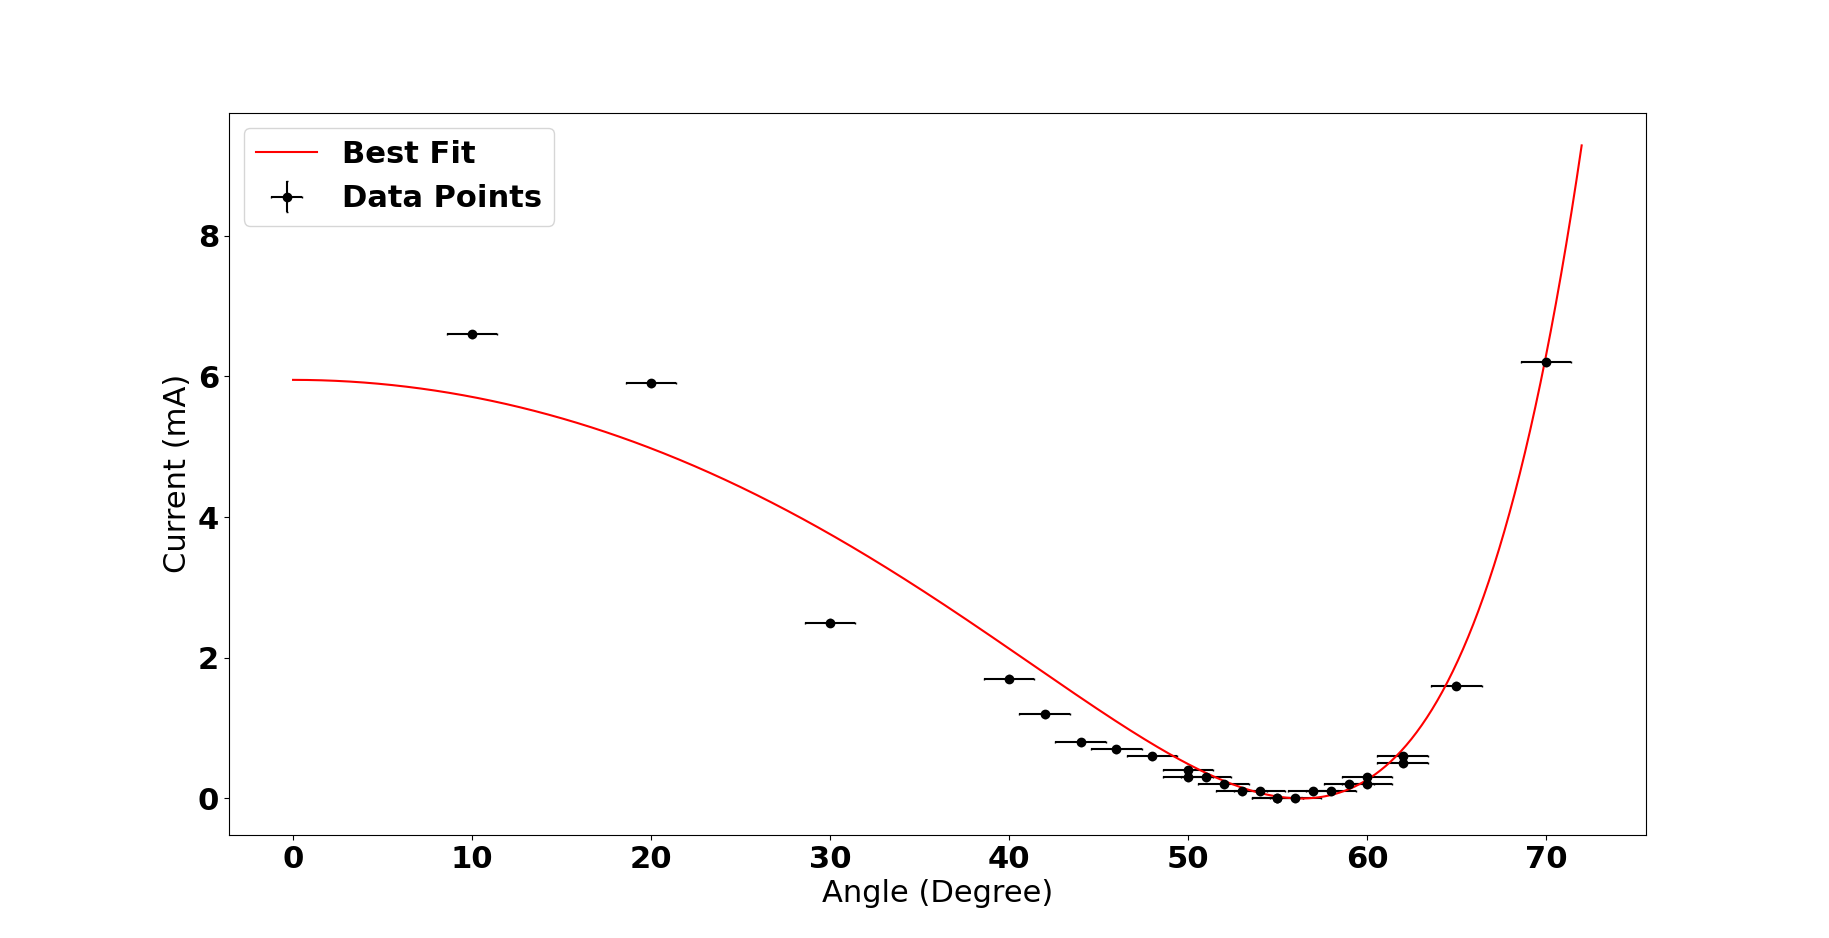
\includegraphics[scale=0.33]{fig}
\caption{Intensity Current vs Angle plot}
\end{figure}\\

From this we get the value of $\eta_1$ and $\eta_2$ to be: 
$$\eta_1 = 1.00034\pm 0.00003 $$ 
$$\eta_2 = 1.50174\pm 0.00004 $$


\subsubsection{Precautions}
\begin{itemize}
	\item Make sure the laser output is larger than the photo detector's input area.
	\item All should lie in the same plane.
	\item All screws should be tight enough so that the laser beam always stays in the plane.
\end{itemize}



\section{Result}
Using weighted mean we get the value of the reflective index as [1][3]:  
\[
\boxed{
\eta_2 = 1.45 \pm 0.05 \eta_1 \\
}
\]
And using Best ODR Fit, we get the value of the reflective index as [1][3]:  

\[
\boxed{
	\eta_1 = 1.00034 \pm 0.00003  \,\,\,\,\,\,
\eta_2 = 1.50174\pm 0.00004
}
\]


\noindent\rule{\linewidth}{0.4pt}
\vspace{3cm}

\bibliographystyle{plain}
\bibliography{bible}

\end{document}
